%%%%%%%%%%%%%%%%%%%%%%%%%%%%%%%%%%%%%%%%%%%%%%%%%%%%%%%%%%%%%%%%%%%%%%%%%%%%%%%%
%2345678901234567890123456789012345678901234567890123456789012345678901234567890
%        1         2         3         4         5         6         7         8


\documentclass[a4paper, 10pt, conference] {article}        
                                                           

%\IEEEoverridecommandlockouts                              % This command is only
                                                          % needed if you want to
                                                          % use the \thanks command
%\overrideIEEEmargins
% See the \addtolength command later in the file to balance the column lengths
% on the last page of the document



% The following packages can be found on http:\\www.ctan.org
\usepackage{graphicx} % for pdf, bitmapped graphics files
\usepackage{caption}
\usepackage{float}
\usepackage{subcaption}
\usepackage{epsfig} % for postscript graphics files
\usepackage{mathptmx} % assumes new font selection scheme installed
\usepackage{times} % assumes new font selection scheme installed
\usepackage{amsmath} % assumes amsmath package installed
\usepackage{amssymb}  % assumes amsmath package installed
\usepackage[margin=1.5cm]{geometry}
\usepackage{mcode}
\usepackage{enumerate}
\begin{document}
\date{}
\title{\LARGE \bf
Programming Assignment 1: Non-linear averaging for image processing
}

\author{ \parbox{5 in}{\centering Daniel Barmaimon \\
%         \thanks{*Use the $\backslash$thanks command to put information here}\\
         \ Advanced Image Analysis - Vibot Master Degree\\
         \ Heriot Watt University\\         
}}

\maketitle
%\thispagestyle{empty}
%\pagestyle{empty}









\section{Introduction}
Since the origins of image processing it has been an increasing interest in finding the best way of locating the edges in the images. The edges could be used in a great variety of applications and very specially in segmentation. There are several algorithms that are able to solve this task, like Canny algorithm or masks based in approximations for the discrete form of the first derivation as Sobel or Prewitt, but they are not accurate when the image is noise or when the image presents textures. Removing the noise or blurring the image to avoid problems with textures will lead to an erosion of the edges. This is due to the use of high pass filter, the noise usually has high frequencies and the edges too. Then the easy and classical average is not useful for our purposes. One way to solve the problem is using a non-linear filter. 


\section{Fundamentals}
The filter should consider if the pixel to study is part of an edge (or surrounded by one) or not, giving a certain weight that will change depending in the intensity values of the neighbourhood to consider. Let consider the following expressions for the definition of the new filter.
\begin{equation}
I_{0}(x,y) = I(x,y)
\end{equation} 
\begin{equation}
I_{n+1}(x,y) = \sum\limits_{i=-1}^1\sum\limits_{j=-1}^1 w_{ij}I_{n}(x+i, y+j)/\sum\limits_{i=-1}^1\sum\limits_{j=-1}^1 w_{ij} 
\end{equation}
\begin{equation}
w_{ij} = exp(-k \left|I_{n}(x,y)-I_{n}(x+i,y+j)\right|)
\end{equation}
In this filter \textit{k} is a positive number, and the variation on this value is going to be one of the two parameters to set.
The other parameter will be the number of iterations, in the case, \textit{n}. The weights for each pixel depends in the variations with respect to the neighbours that surround, for each iteration. 

\section{Evaluation and analysis}
\subsection{Analysis of \textit{k} variation}
First evaluation was made over the different values of \textit{k}. It will affect the weight, making the filter effect weaker as this value is increased. The effects could be appreciated in the image \ref{kanalysis}. 
\begin{figure}[H]
	\centering
	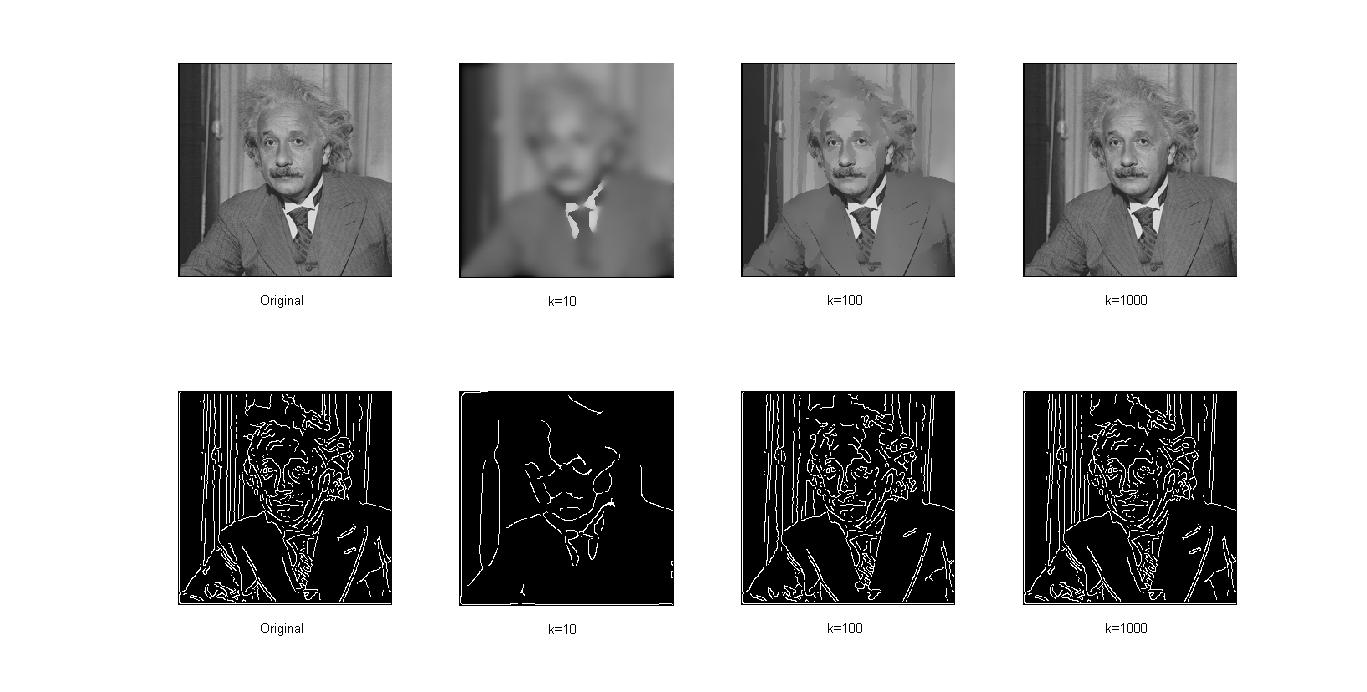
\includegraphics[width=1\textwidth]{analysis_einstein_k.JPG} %
	\caption{Effects of varying \textit{k} over the image  for 50 iterations}
	\label{kanalysis}
\end{figure}

It can be appreciated the differences in the two central images, where some areas have been smoothed while the edges could still been detected. An edge detection have been applied to the same images to check with detail the effects when \textit{k} varies. If \textit{k} is too big, the effects of the filter over the image are negligible. 

\subsection{Analysis of \textit{n}, number of iterations}
The number of iterations is the second parameter that should be set for a good performance of the filter. The bigger the number of iterations the more homogeneous will be the areas that compound the image, but also much more computational expensive.  
\begin{figure}[H]
	\centering
	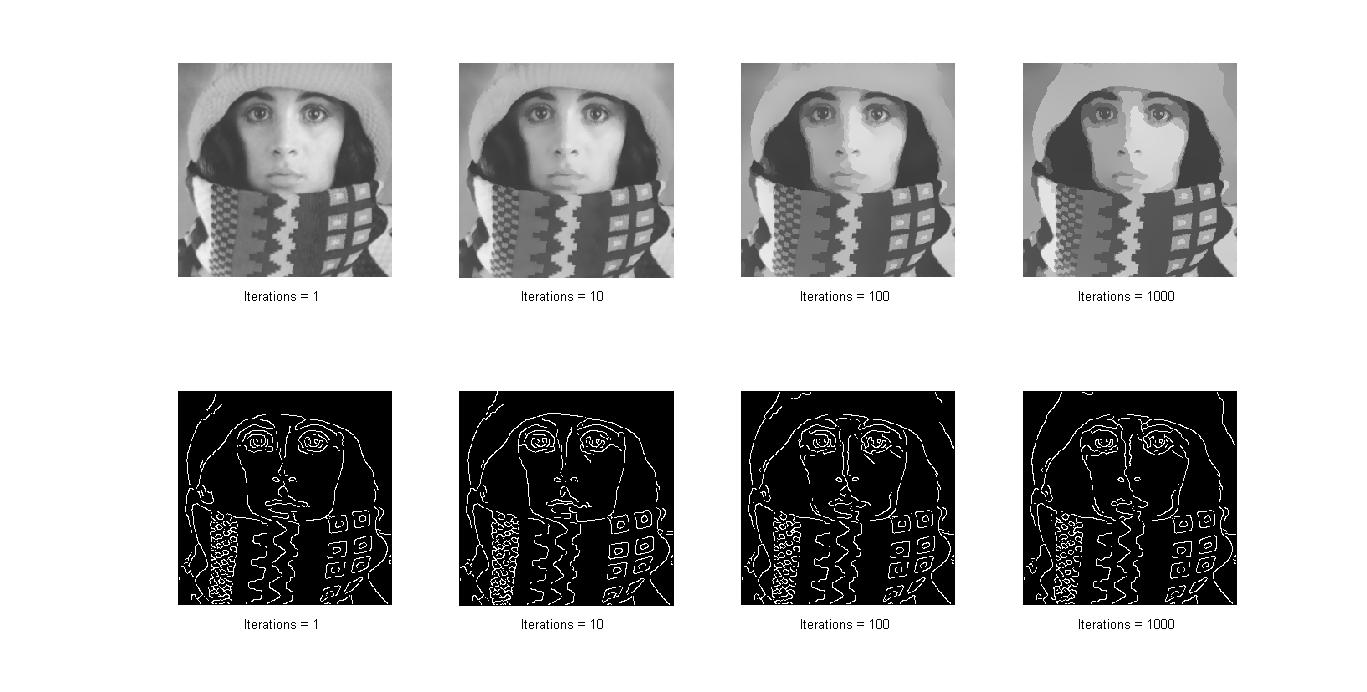
\includegraphics[width=1\textwidth]{analysis_trui_it.JPG} %
	\caption{Effects of varying \textit{n}, nº of iterations for \textit{k}=100}
	\label{itanalysis}
\end{figure}
In the Fig.\ref{itanalysis}, several experiments with different number of iterations were performed. For a deeper analysis a mesh plot over a small area of the same image will be shown in Fig.\ref{mesh}.

 \begin{figure}[H]
 	\centering
 	\begin{subfigure}{0.29\textwidth} 						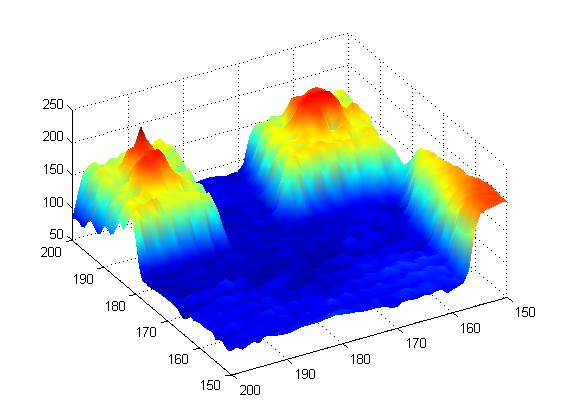
\includegraphics[scale=0.300]{mesh_original.JPG}
		\caption{Original}
	\end{subfigure}
	\begin{subfigure}{0.29\textwidth} 						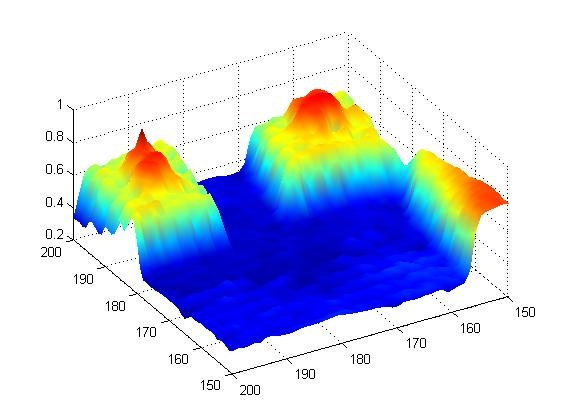
\includegraphics[scale=0.300]{mesh_solution1.JPG}
		\caption{\textit{n}= 1 Iteration}
	\end{subfigure}
	\begin{subfigure}{0.29\textwidth} 						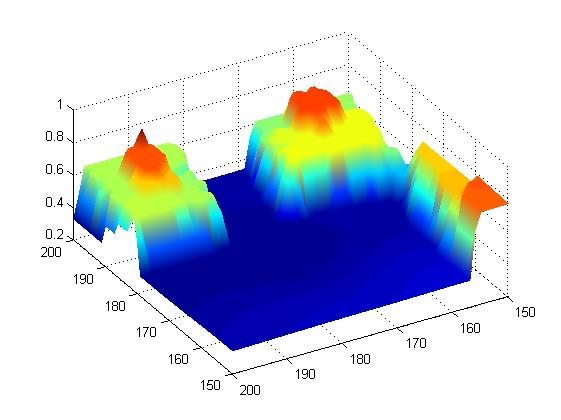
\includegraphics[scale=0.300]{mesh_solution3.JPG}
		\caption{\textit{n}= 100 Iterations}
	\end{subfigure}
	\caption{Analysis with mesh grid plot for [125:200 ;125:200] for 'trui.tif'and \textit{k}=100}
	\label{mesh}
\end{figure}
	
As a simple example of how much the noise can be reduce and how good it could be for segmentation purposes the region growing algorithm was implemented over two different images, as is reflected in Fig.\ref{regionGrowing}
\begin{figure}[H]
 	\centering
 	\begin{subfigure}{0.45\textwidth} 						
 	\centering
 	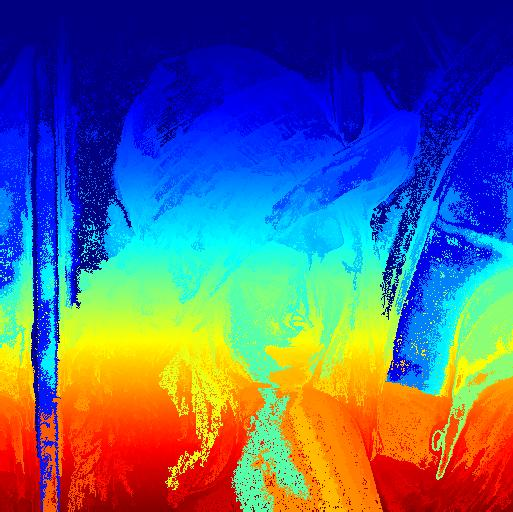
\includegraphics[scale=0.35]{original_segmented.JPG}
		\caption{Original image}
	\end{subfigure}
	\begin{subfigure}{0.45\textwidth}
	\centering
	 						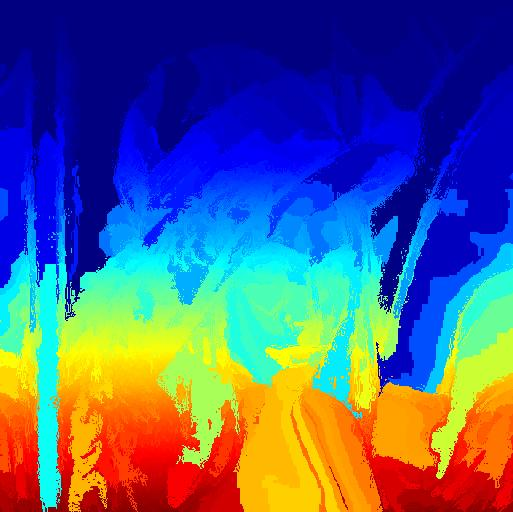
\includegraphics[scale=0.35]{filtered_segmented.JPG}
		\caption{\textit{n}= 100 iterations, \textit{k}= 100}
	\end{subfigure}
	\caption{Region growing segmentation analysis}
	\label{regionGrowing}
\end{figure}

%\begin{figure}[ht!]
%  \centering
%  \includegraphics[width=0.5\textwidth]{delta_qVsTime.jpg}
%  \caption{Average time of computation versus step size}
%  \label{timeVSstep}
%\end{figure}

The results shows a great reduction of the noise for the filtered image. The information of the edges is remaining but special care should be taken with the illumination sources and its effects over the filtered image.





% \begin{figure}[ht!]
% \centering
% \includegraphics[width=1\textwidth]{pseudoCode.JPG}
% \caption{Pseudo code for the A* algorithm representation}
% \label{pseudo}
% \end{figure}
%\clearpage 
%\section{Experiments}
%The implementation was quite straight forward using the pseudo code and having care to check the visibility in both directions. Until the path is found, the list of nodes that were checked and the ones to be considered are added into two different lists. The distances from last vertex, and the distance to the goal where checked and used as conditions to validate a new point of the path or to start to search in another branch.
%
%The results over two different environments are shown below. The environment is given by the vertices and the object they below to. The visibility for each environment is given. It is pretended to get to the last vertex from the first one by the shortest possible path.
%
%  \begin{figure}[ht!]
%  \begin{subfigure}{0.5\textwidth}
%  \centering
% \includegraphics{A.JPG}
%  \caption{Vertices coordintes and vertices for small environment}
%  \label{A}
%  \end{subfigure}
%  \begin{subfigure}{0.5\textwidth}
%  \centering
%  \includegraphics[scale=0.4]{small_environment.JPG}
%  \caption{Graphic plot of the results}
%  \label{resA}
%  \end{subfigure}\\
% 
%  \begin{subfigure}{0.5\textwidth}
%  \centering
%  \includegraphics[scale=0.8]{small_results.JPG}
%  \caption{List of visible combination for vertices}
%  \label{numA}
%  \end{subfigure}
%  \begin{subfigure}{0.5\textwidth}
%  \includegraphics[scale=0.8]{pathA.JPG}
%  \caption{Results for optimal path in small environment}
%  \label{pathA}
%  \end{subfigure}
%  \end{figure} 
%\clearpage
% \begin{figure}[ht!]
%  \begin{subfigure}{0.5\textwidth}
%  \centering
% \includegraphics{B.JPG}
%  \caption{Vertices coordintes and vertices for big environment}
%  \label{B}
%  \end{subfigure}
%  \begin{subfigure}{0.4\textwidth}
%  \includegraphics[scale=0.6]{big_environment.JPG}
%  \caption{Graphic plot of the results}
%  \label{resB}
%  \end{subfigure}\\
%
% 	\begin{tabular}{ c c c c}
%   	\begin{subfigure}{0.1\textwidth}
%   	        \centering
%   	         \includegraphics[scale=0.7]{big_results_01.JPG}
%   	          \label{numB1}
%   	\end{subfigure}&
%   	\begin{subfigure}{0.1\textwidth}
%   	  	        \centering
%   	  	         \includegraphics[scale=0.7]{big_results_02.JPG}
%   	  	         \label{numB2}
%   	  	\end{subfigure}&
%   	  	\begin{subfigure}{0.1\textwidth}
%   	  	  	        \centering
%   	  	  	         \includegraphics[scale=0.7]{big_results_03.JPG}
%   	  	  	          \label{numB3}
%   	  	  	\end{subfigure}& ~~~~~~~~~~~~~~~~~~~~~~~~~~~~~~ 
%   	  	  	\begin{subfigure}{\textwidth}
%   	  	  	  	  \includegraphics[scale=1]{pathB.JPG}
%   	  	  	  	  
%   	  	  	  	  \end{subfigure}
%  	\end{tabular}~~
%%  	\begin{subfigure}{0.5\textwidth}
%%  	  \includegraphics[scale=0.8]{pathB.JPG}
%%  	  \caption{Results for optimal path in big environment}
%%  	  \label{pathB}
%%  	  \end{subfigure}
%    	
%    	
%  
%  \end{figure} 
  

\begin{thebibliography}{99}
%%
\bibitem{c1}
Perona, Pietro, and Jitendra Malik. "Scale-space and edge detection using anisotropic diffusion." Pattern Analysis and Machine Intelligence, IEEE Transactions on 12.7 (1990): 629-639.
\bibitem{c2}
'Advanced Image Analysis Notes', Alexander Belyaev, Heriot Watt University, 2014
%%
%%\bibitem{c3}
%%'Ultrasound Image Enhancement Based on Image Compounding' - Yair Kerner - Technion (Israel Institute of Technology) - Haifa - June 2004 
%%
%%\bibitem{c4}
%%'Physical Principles of General and Vascular Sonography' - Jim Baun - San Francisco, CA -March 2009
%%
%%\bibitem{c5}
%%'Physical Principles of General and Vascular Sonography' - Jim Baun - San Francisco, CA -March 2009
%%
%%\bibitem{c6}
%%'Image Formation and Image Processing in Ultrasound' - Jeffrey C. Bamber - Institute of Cancer Research and The Royal Marsden NHS Trust, Surrey, SM2 5PT
\end{thebibliography}

\end{document}
